\documentclass[11pt]{amsart}
\usepackage[T1]{fontenc}
\usepackage{lmodern}
\usepackage{amsmath,amssymb,amsthm,mathtools}
\usepackage{microtype}
\usepackage{booktabs}
\usepackage{tikz}
\usepackage{pgfplots}
\pgfplotsset{compat=1.17}
\usepackage[colorlinks=true,linkcolor=blue!50!black,citecolor=blue!50!black,urlcolor=blue!50!black]{hyperref}

\newtheorem{theorem}{Theorem}[section]
\newtheorem{proposition}[theorem]{Proposition}
\newtheorem{lemma}[theorem]{Lemma}
\newtheorem{corollary}[theorem]{Corollary}
\theoremstyle{definition}
\newtheorem{definition}[theorem]{Definition}
\newtheorem{example}[theorem]{Example}
\theoremstyle{remark}
\newtheorem{remark}[theorem]{Remark}

\DeclareMathOperator{\re}{Re}
\DeclareMathOperator{\im}{Im}
\DeclareMathOperator*{\res}{Res}
\newcommand{\C}{\mathbb{C}}
\newcommand{\R}{\mathbb{R}}
\newcommand{\Z}{\mathbb{Z}}
\newcommand{\cL}{\mathcal{L}}
\newcommand{\M}{\mathsf{M}}
\newcommand{\lean}[1]{\texttt{#1}}
\newcommand{\dd}{\,\mathrm{d}}

\title[A pole in the critical strip survives the mix $-1,3,-2$]{Why a pole in the critical strip survives\\ the delayed second difference with weights $-1,\,3,\,-2$}

\author{Math-To-Manim Mythos chain}
\thanks{Expository companion to the film \emph{The Mix That Cannot Kill a Pole}. The film, this
paper and the Lean file \lean{DelayedPoleSurvival.lean} were produced in one run of the Mythos
chain of Math-To-Manim, with Claude Fable~5.2 as the operator of the chain. The transfer theorem
(Theorem~\ref{thm:transfer}) is due to L.~Crossley~\cite{Crossley-transfer}; the proofs of
Section~\ref{sec:transfer} follow his Lean file. Set the author line before any submission.}

\date{22 November 2026}

\subjclass[2020]{Primary 11M26; Secondary 44A10, 30D10, 68V20}
\keywords{Laplace transform, delay, exponential polynomial, pole, residue, critical strip, Lean}

\begin{document}

\begin{abstract}
Take a function $g$ on the half-line, form three copies, delay two of them by $\log 2$ and $\log 4$,
and add the copies with weights $-1$, $3$ and $-2$. On the Laplace side this operation is the
multiplication by the exponential polynomial $m(s)=-1+3\cdot 2^{-s}-2\cdot 4^{-s}
=(1-2^{-s})(2\cdot 2^{-s}-1)$. We give a complete account of why a simple pole of the
transform at a point $\rho$ with $0<\re\rho<1$ survives: the zeros of $m$ are exactly the points
$2\pi i k/\log 2$ and $1+2\pi i k/\log 2$, $k\in\Z$, so they lie on the two boundary lines of the
strip, and the residue is multiplied by $m(\rho)\neq 0$. We add three quantitative complements: the
sharp bounds $(1-2^{-\sigma})(2^{1-\sigma}-1)\le |m(\sigma+it)|\le(1+2^{-\sigma})(2^{1-\sigma}+1)$,
the identification of the two boundary zeros with the compact support of the associated tent weight,
and a worked example at the first zero of the Riemann zeta function, where $|m(\rho_1)|=3.984040$.
The statement is the analytic step in a delayed-difference window criterion of
Crossley~\cite{Crossley-transfer}. All statements of Sections~\ref{sec:symbol}--\ref{sec:tent}
are checked in Lean~4 with Mathlib. Nothing here proves a zero-free region or the Riemann hypothesis.
\end{abstract}

\maketitle

\section{Introduction}

\subsection{The question}
Let $c=\log 2$. For a function $g\colon\R\to\R$ and $a\ge 0$ let
\[
(\tau_a g)(u)=\begin{cases} g(u-a), & u>a,\\ 0, & u\le a,\end{cases}
\]
be the copy of $g$ delayed by $a$ and extended by zero. The \emph{mix} of $g$ is
\begin{equation}\label{eq:mix}
\begin{aligned}
\M g&=-\tau_0 g+3\,\tau_{c}\,g-2\,\tau_{2c}\,g,\\
(\M g)(u)&=-g(u)+3g(u-\log 2)-2g(u-\log 4)\qquad (u>\log 4).
\end{aligned}
\end{equation}
Suppose that the one-sided Laplace transform $\Phi(s)=\int_0^\infty g(u)e^{-su}\dd u$ continues
meromorphically and has a simple pole at a point $\rho$ with $0<\re\rho<1$. The weights of the mix
sum to zero, so the mix is built to cancel. \emph{Does it cancel the pole?}

\subsection{The answer}
No. The Laplace transform of $\M g$ is $m(s)\Phi(s)$ with
\begin{equation}\label{eq:symbol}
m(s)=-1+3\cdot 2^{-s}-2\cdot 4^{-s}=(1-q)(2q-1),\qquad q=2^{-s}.
\end{equation}
The quadratic $-1+3q-2q^2$ vanishes only at $q=1$ and $q=\tfrac12$. Because $|q|=2^{-\re s}$,
the strip $0<\re s<1$ is mapped into the open annulus $\tfrac12<|q|<1$, and the two roots lie on the
boundary circles of that annulus (Figure~\ref{fig:annulus}). Hence $m(\rho)\ne0$, and
$m\Phi$ has a simple pole at $\rho$ with residue $m(\rho)\res_{s=\rho}\Phi$.

The same computation, read in the $u$ variable, says that each exponential $e^{\rho u}$ is an
eigenfunction of the mix with eigenvalue $m(\rho)$ (Proposition~\ref{prop:modes}). A pole of $\Phi$ at
$\rho$ is the transform's record of a term $r\,e^{\rho u}$ in $g$, and the mix returns
$m(\rho)\,r\,e^{\rho u}$. The mix removes exactly the modes with $2^{-\rho}\in\{1,\tfrac12\}$:
constants, the growth $e^{u}$, and their translates by $2\pi i k/\log 2$.

\subsection{Context}
The statement is the analytic step of Crossley's delayed-difference window
criterion~\cite{Crossley-transfer}. There $g$ is the observable attached to a family of Dirichlet
$L$-functions, the poles of $\Phi$ sit at the zeros of the members of the family, and a
Landau-type theorem from an upstream source release~\cite{upstream} turns a one-sided bound for a
function with pole data into the absence of poles with large real part. The mix replaces a
non-compact weight by a compactly supported tent (Section~\ref{sec:tent}). For the criterion to
remain usable, the mix must keep every pole. That is Theorem~\ref{thm:transfer}, which is
\lean{compactDifference\_poleData} in~\cite{Crossley-transfer}; a specialisation to a sum over
primes is in~\cite{Crossley-prime}.

\subsection{What this paper adds}
The theorem is not new. This paper gives its proof in ordinary mathematical language, and adds:
the exact zero set of $m$ (Proposition~\ref{prop:zeros}); sharp lower and upper bounds for $|m|$ on
vertical lines (Proposition~\ref{prop:bounds}), which bound the change of each residue
(Theorem~\ref{thm:pole}); the remark that the two boundary zeros are forced by the compact support
of the tent (Proposition~\ref{prop:mellin}); an example of a two-term mix that \emph{does} remove
poles on the critical line (Remark~\ref{rem:kills}); and a numerical example
(Section~\ref{sec:example}). Section~\ref{sec:lean} lists the Lean names of the statements.

\begin{figure}[t]
\centering
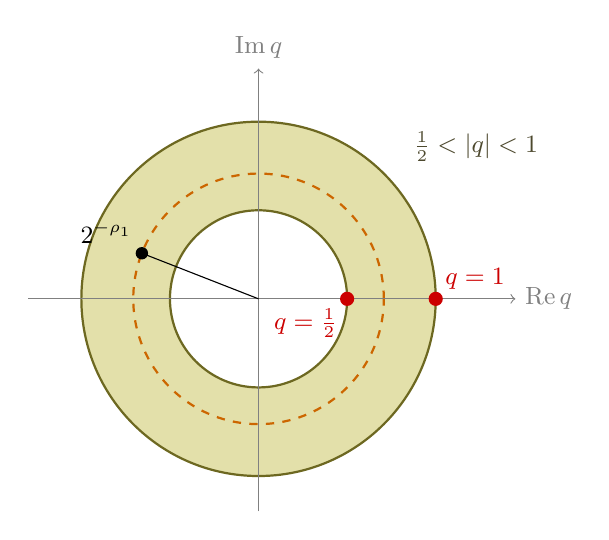
\begin{tikzpicture}[scale=2.25]
  \fill[olive!25] (0,0) circle (1);
  \fill[white] (0,0) circle (0.5);
  \draw[olive!70!black, thick] (0,0) circle (1);
  \draw[olive!70!black, thick] (0,0) circle (0.5);
  \draw[orange!80!black, thick, dashed] (0,0) circle (0.7071);
  \draw[->, gray] (-1.3,0) -- (1.45,0) node[right] {\small $\re q$};
  \draw[->, gray] (0,-1.2) -- (0,1.3) node[above] {\small $\im q$};
  \fill[red!80!black] (1,0) circle (0.04) node[above right] {\small $q=1$};
  \fill[red!80!black] (0.5,0) circle (0.04) node[below left] {\small $q=\tfrac12$};
  \fill[black] (-0.6586,0.2575) circle (0.035) node[above left] {\small $2^{-\rho_1}$};
  \draw[black, thin] (0,0) -- (-0.6586,0.2575);
  \node[olive!40!black, anchor=west] at (0.82,0.86) {\small $\tfrac12<|q|<1$};
\end{tikzpicture}
\caption{The $q$-plane, $q=2^{-s}$. The strip $0<\re s<1$ is mapped into the shaded open annulus.
The two zeros of $(1-q)(2q-1)$ lie on its boundary circles. The dashed circle $|q|=2^{-1/2}$ is the
image of the critical line; the black point is $2^{-\rho_1}$ for the first zeta zero
$\rho_1=\tfrac12+14.134725\,i$.}
\label{fig:annulus}
\end{figure}

\section{Notation and the transform of the mix}\label{sec:laplace}

Throughout, $c=\log 2$, $s=\sigma+it$ with $\sigma,t\in\R$, and $q=q(s)=e^{-sc}=2^{-s}$.
For measurable $g\colon\R\to\C$ and $s\in\C$ with $\int_0^\infty|g(u)|e^{-\sigma u}\dd u<\infty$ we write
$\cL g(s)=\int_0^\infty g(u)e^{-su}\dd u$.

\begin{lemma}[A delay is a multiplication]\label{lem:delay}
Let $a\ge0$ and let $g$ be measurable with $\int_0^\infty|g(u)|e^{-\sigma u}\dd u<\infty$. Then
$\int_0^\infty|\tau_ag(u)|e^{-\sigma u}\dd u<\infty$ and
\[
\cL(\tau_a g)(s)=e^{-sa}\,\cL g(s).
\]
\end{lemma}

\begin{proof}
Since $\tau_ag$ vanishes on $(0,a]$, the substitution $u=v+a$ gives
\begin{align*}
\int_0^\infty \tau_ag(u)e^{-su}\dd u&=\int_a^\infty g(u-a)e^{-su}\dd u\\
&=\int_0^\infty g(v)e^{-s(v+a)}\dd v=e^{-sa}\cL g(s).
\end{align*}
The same substitution with absolute values gives the integrability, with the factor
$e^{-\sigma a}\le 1$.
\end{proof}

\begin{proposition}[The mix is a multiplication]\label{prop:symbol}
Let $g$ be measurable with $|g(u)|\le Ce^{2u}$ for $u\ge0$. Then $|\M g(u)|\le 6Ce^{2u}$ for
$u\ge 0$, and for $\re s>2$
\[
\cL(\M g)(s)=m(s)\,\cL g(s),\qquad m(s)=-1+3e^{-sc}-2e^{-2sc}=(1-q)(2q-1).
\]
\end{proposition}

\begin{proof}
For $a\ge0$ and $u>a$ we have $|\tau_ag(u)|\le Ce^{2(u-a)}\le Ce^{2u}$, and $\tau_ag(u)=0$ for
$u\le a$; this gives the bound with $1+3+2=6$. For $\re s>2$ all three integrals converge
absolutely, so Lemma~\ref{lem:delay} and linearity give
$\cL(\M g)=(-1+3e^{-sc}-2e^{-2sc})\cL g$. Finally $(1-q)(2q-1)=2q-1-2q^2+q=-1+3q-2q^2$ and
$e^{-2sc}=q^2$.
\end{proof}

\begin{remark}[Convolution form]\label{rem:convolution}
If $g$ vanishes on $(-\infty,0]$, then $\M g=g*\mu$ with the measure
$\mu=-\delta_0+3\delta_{c}-2\delta_{2c}$, and $m(s)=\int e^{-sa}\dd\mu(a)$ is the Laplace transform
of $\mu$. So $m$ is an exponential polynomial with the three frequencies $0$, $c$, $2c$. They are
commensurable; this is why $m$ is a polynomial in the single variable $q$ and why its zero set
is a union of two arithmetic progressions on two vertical lines.
\end{remark}

\begin{proposition}[Exponentials are eigenfunctions]\label{prop:modes}
For $\lambda\in\C$ put $e_\lambda(u)=e^{\lambda u}$. Then for $u>2c$,
\[
(\M e_\lambda)(u)=m(\lambda)\,e^{\lambda u}.
\]
In particular $\M$ annihilates the constants and the function $e^{u}$ on $(2c,\infty)$:
$m(0)=-1+3-2=0$ and $m(1)=-1+\tfrac32-\tfrac24=0$.
\end{proposition}

\begin{proof}
For $u>2c$ all three delays have started, so
$(\M e_\lambda)(u)=-e^{\lambda u}+3e^{\lambda(u-c)}-2e^{\lambda(u-2c)}
=(-1+3e^{-\lambda c}-2e^{-2\lambda c})e^{\lambda u}$.
\end{proof}

\section{The symbol and its zeros}\label{sec:symbol}

\begin{lemma}\label{lem:radius}
$|q(s)|=2^{-\sigma}$ and $\arg q(s)\equiv -t\log 2 \pmod{2\pi}$. If $0<\sigma<1$ then
$\tfrac12<|q(s)|<1$.
\end{lemma}

\begin{proof}
$q=e^{-(\sigma+it)c}=e^{-\sigma c}e^{-itc}$. The function $\sigma\mapsto 2^{-\sigma}$ is strictly
decreasing with values $1$ at $\sigma=0$ and $\tfrac12$ at $\sigma=1$.
\end{proof}

\begin{proposition}[The zero set]\label{prop:zeros}
$m(s)=0$ if and only if
\[
s=\frac{2\pi i k}{\log 2}\quad\text{or}\quad s=1+\frac{2\pi i k}{\log 2}\qquad\text{for some }k\in\Z .
\]
All zeros are simple. In particular every zero of $m$ has real part $0$ or $1$, and
$m(s)\neq0$ for $0<\re s<1$.
\end{proposition}

\begin{proof}
By \eqref{eq:symbol}, $m(s)=0$ if and only if $q=1$ or $q=\tfrac12$. Now $e^{-sc}=1$ if and only if
$-sc\in 2\pi i\Z$, and $e^{-sc}=\tfrac12=e^{-c}$ if and only if $-sc+c\in2\pi i\Z$. This gives the
two progressions. For the multiplicity, $\tfrac{\mathrm d}{\mathrm ds}q=-cq$, hence
\begin{equation}\label{eq:derivative}
m'(s)=-cq\bigl(-(2q-1)+2(1-q)\bigr)=-cq\,(3-4q),
\end{equation}
which equals $c$ at $q=1$ and $-\tfrac c2$ at $q=\tfrac12$. The last assertion also follows from
Lemma~\ref{lem:radius}: inside the strip $|q|\ne1$ and $|q|\ne\tfrac12$.
\end{proof}

The spacing of the zeros on each line is $2\pi/\log2=9.064720\ldots$.

\begin{proposition}[Sharp bounds on vertical lines]\label{prop:bounds}
Let $0\le\sigma\le1$ and put $x=2^{-\sigma}\in[\tfrac12,1]$. For every $t\in\R$,
\begin{equation}\label{eq:bounds}
\varphi(\sigma):=(1-x)(2x-1)\ \le\ |m(\sigma+it)|\ \le\ (1+x)(2x+1).
\end{equation}
Equality holds on the left exactly when $t\in\frac{2\pi}{\log 2}\Z$, and on the right exactly when
$t\in\frac{2\pi}{\log 2}\bigl(\Z+\tfrac12\bigr)$. The function $\varphi$ is positive on $(0,1)$,
vanishes at $0$ and $1$, and has its maximum $\tfrac18$ at $\sigma=\log_2\tfrac43=0.415037\ldots$.
On the critical line, $\varphi(\tfrac12)=\tfrac{3}{\sqrt2}-2=0.121320\ldots$ and the upper bound is
$\tfrac{3}{\sqrt2}+2=4.121320\ldots$.
\end{proposition}

\begin{proof}
Write $q=xe^{i\theta}$ with $\theta=-t\log2$. By the triangle inequality,
$1-x\le|1-q|\le1+x$ and $2x-1\le|2q-1|\le2x+1$; note that $1-x\ge0$ and $2x-1\ge0$. Multiplying
gives \eqref{eq:bounds}. In $|1-q|\ge 1-|q|$ equality holds if and only if $q\ge0$, and in
$|2q-1|\ge2|q|-1$ (with $2|q|\ge1$) equality holds if and only if $q\ge 0$. Since $x>0$, both hold
exactly when $e^{i\theta}=1$. The two upper inequalities are equalities exactly when
$e^{i\theta}=-1$. For the maximum, $(1-x)(2x-1)=-2x^2+3x-1$ is maximal at $x=\tfrac34$ with value
$\tfrac18$. At $x=2^{-1/2}$, $(1-x)(2x-1)=3x-1-2x^2=\tfrac{3}{\sqrt2}-2$ and
$(1+x)(2x+1)=3x+1+2x^2=\tfrac{3}{\sqrt2}+2$.
\end{proof}

\begin{corollary}[Real points]\label{cor:real}
If $0<\sigma<1$ then $m(\sigma)=\varphi(\sigma)>0$.
\end{corollary}

\begin{proof}
For real $s=\sigma$ the number $q=2^{-\sigma}$ is real, with $\tfrac12<q<1$, so both factors of
$(1-q)(2q-1)$ are positive.
\end{proof}

\begin{figure}[t]
\centering
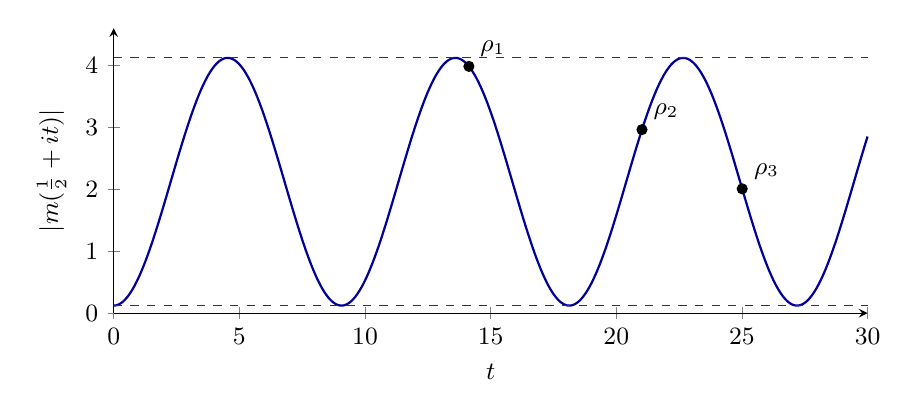
\begin{tikzpicture}
\begin{axis}[width=0.92\textwidth, height=5.2cm, xmin=0, xmax=30, ymin=0, ymax=4.6,
  xlabel={$t$}, ylabel={$|m(\tfrac12+it)|$}, samples=400, domain=0:30,
  axis lines=left, tick label style={font=\small}, label style={font=\small},
  ytick={0,1,2,3,4}, clip=false]
  \addplot[blue!60!black, thick]
    {sqrt((1.5 - 1.41421356*cos(deg(0.69314718*x))) * (3 - 2.82842712*cos(deg(0.69314718*x))))};
  \addplot[red!70!black, dashed, domain=0:30, samples=2] {0.12132};
  \addplot[red!70!black, dashed, domain=0:30, samples=2] {4.12132};
  \addplot[only marks, mark=*, mark size=1.8pt, black] coordinates
    {(14.134725,3.984040) (21.022040,2.962691) (25.010858,2.006492)};
  \node[font=\small, anchor=south west] at (axis cs:14.2,3.99) {$\rho_1$};
  \node[font=\small, anchor=south west] at (axis cs:21.1,2.97) {$\rho_2$};
  \node[font=\small, anchor=south west] at (axis cs:25.1,2.01) {$\rho_3$};
\end{axis}
\end{tikzpicture}
\caption{The modulus of the symbol on the critical line. It is periodic with period
$2\pi/\log 2=9.0647$ and stays between the dashed lines $\tfrac{3}{\sqrt2}\mp2$ of
Proposition~\ref{prop:bounds}. The marked points are the first three zeros of $\zeta$.}
\label{fig:critical}
\end{figure}

\section{The pole survives}\label{sec:pole}

\begin{lemma}[An analytic multiplier and a simple pole]\label{lem:multiplier}
Let $\rho\in\C$, let $h$ and $M$ be analytic in a neighbourhood $U$ of $\rho$, let $r\in\C$, and let
$\Phi(s)=\dfrac{r}{s-\rho}+h(s)$ on $U\setminus\{\rho\}$. Then on $U\setminus\{\rho\}$
\[
M(s)\Phi(s)=\frac{M(\rho)\,r}{s-\rho}+\tilde h(s),\qquad
\tilde h(s)=M(s)h(s)+r\,\frac{M(s)-M(\rho)}{s-\rho},
\]
and $\tilde h$ extends analytically to $\rho$, with $\tilde h(\rho)=M(\rho)h(\rho)+r\,M'(\rho)$.
Consequently $M\Phi$ has at $\rho$ a simple pole with residue $M(\rho)r$ if $M(\rho)r\ne0$, and a
removable singularity otherwise.
\end{lemma}

\begin{proof}
The identity is $M(s)r=M(\rho)r+r\,(M(s)-M(\rho))$ divided by $s-\rho$. The difference quotient
$(M(s)-M(\rho))/(s-\rho)$ has a removable singularity at $\rho$ with value $M'(\rho)$.
\end{proof}

\begin{theorem}[The pole survives the mix]\label{thm:pole}
Let $0<\re\rho<1$, let $h$ be analytic near $\rho$, $r\neq 0$, and
$\Phi(s)=\dfrac{r}{s-\rho}+h(s)$ near $\rho$. Then $m\Phi$ has a simple pole at $\rho$, with
\begin{gather*}
\res_{s=\rho}\,m\Phi=m(\rho)\,r\neq0,\\
\varphi(\re\rho)\,|r|\ \le\ |m(\rho)\,r|\ \le\ \bigl(1+2^{-\re\rho}\bigr)\bigl(2^{1-\re\rho}+1\bigr)|r| .
\end{gather*}
If $\rho$ is real and $r>0$, then $m(\rho)\,r>0$.
\end{theorem}

\begin{proof}
The symbol $m$ is entire, so Lemma~\ref{lem:multiplier} applies with $M=m$. By
Proposition~\ref{prop:zeros}, $m(\rho)\ne0$. The bounds are Proposition~\ref{prop:bounds} and the
last statement is Corollary~\ref{cor:real}.
\end{proof}

\begin{remark}[What happens on the walls]\label{rem:walls}
If $\Phi$ has a simple pole at a zero of $m$, for instance at $s=0$ or $s=1$, then by
Lemma~\ref{lem:multiplier} the product $m\Phi$ is analytic there: the mix removes that pole. By
Proposition~\ref{prop:modes} this is the statement that the mix annihilates the corresponding mode.
A double pole at a zero of $m$ becomes a simple pole, because the zeros of $m$ are simple.
\end{remark}

\begin{remark}[A mix that does kill]\label{rem:kills}
The conclusion of Theorem~\ref{thm:pole} is a property of the weights. The two-term mix
$g\mapsto \tau_0g-\sqrt2\,\tau_cg$ has the symbol $1-\sqrt2\,q$, which vanishes when
$q=2^{-1/2}$, that is at $s=\tfrac12+2\pi ik/\log2$, $k\in\Z$. These points are on the critical
line, and a pole of $\Phi$ at one of them would be removed. In general a mix with weights $w_j$ and
delays $jc$ has the symbol $P(q)=\sum_jw_jq^j$, and a simple pole at $\rho$ survives if and only if
$P(2^{-\rho})\ne0$. Up to a scalar, $-1+3q-2q^2=-2(q-1)(q-\tfrac12)$ is the only quadratic whose
roots are $1$ and $\tfrac12$. Section~\ref{sec:tent} explains why these two roots are needed.
\end{remark}

\section{What the weights are for: the tent}\label{sec:tent}

Let $x_+=\max(x,0)$. For $t>0$ define
\begin{equation}\label{eq:tent}
W(t)=\Bigl(\frac4t-1\Bigr)_{\!+}-3\Bigl(\frac2t-1\Bigr)_{\!+}+2\Bigl(\frac1t-1\Bigr)_{\!+}.
\end{equation}

\begin{lemma}[The tent]\label{lem:tent}
$W(t)=0$ for $t\le1$ and for $t\ge4$, $W(t)=2\bigl(1-\tfrac1t\bigr)$ for $1<t\le2$, and
$W(t)=\tfrac4t-1$ for $2<t<4$. So $W$ is continuous, non-negative, supported in $[1,4]$, with
$W(2)=1$.
\end{lemma}

\begin{proof}
For $t\le1$ all three brackets are non-negative and
$(\tfrac4t-1)-3(\tfrac2t-1)+2(\tfrac1t-1)=\tfrac{4-6+2}{t}+(-1+3-2)=0$. For $1<t\le2$ the third
bracket is negative and $(\tfrac4t-1)-3(\tfrac2t-1)=2-\tfrac2t$. For $2<t<4$ only the first
bracket is positive. For $t\ge4$ none is.
\end{proof}

The cancellation for $t\le 1$ uses both relations $-1+3-2=0$ and $4-6+2=0$; in the variable $q$
these are $m(0)=0$ and $m(1)=0$ after multiplication by $-1$ and by $-4$.

\begin{proposition}[Compact support forces the two boundary zeros]\label{prop:mellin}
For every $s\in\C\setminus\{0,1\}$,
\[
W^*(s):=\int_0^\infty W(t)\,t^{s-1}\dd t=-\frac{4^{s}\,m(s)}{s(s-1)} .
\]
The left side is an entire function of $s$, so the zeros of $m$ at $s=0$ and $s=1$ are exactly
what cancels the two poles of $1/(s(s-1))$. Moreover $W^*(1)=\int_1^4W(t)\dd t=2\log 2$.
\end{proposition}

\begin{proof}
For $a>0$ and $\re s>1$,
$\int_0^\infty(\tfrac at-1)_+t^{s-1}\dd t=\int_0^a(at^{s-2}-t^{s-1})\dd t
=\tfrac{a^s}{s-1}-\tfrac{a^s}{s}=\tfrac{a^s}{s(s-1)}$.
Hence, for $\re s>1$,
$W^*(s)=\dfrac{4^s-3\cdot2^s+2}{s(s-1)}=\dfrac{4^s(1-3\cdot2^{-s}+2\cdot4^{-s})}{s(s-1)}
=-\dfrac{4^sm(s)}{s(s-1)}$. By Lemma~\ref{lem:tent}, $W$ is bounded with support in $[1,4]$, so
$W^*$ is entire, and the identity extends to $\C\setminus\{0,1\}$ by analytic continuation. At
$s=1$, by \eqref{eq:derivative}, $m'(1)=-\tfrac c2$, so the right side tends to
$-4m'(1)=2\log2$. Directly,
$\int_1^2 2(1-\tfrac1t)\dd t+\int_2^4(\tfrac4t-1)\dd t=(2-2\log2)+(4\log2-2)=2\log 2$.
\end{proof}

\begin{example}[The zeta case]\label{ex:zeta}
Let $\Lambda$ be the von Mangoldt function and $R(y)=\sum_{n}\Lambda(n)\bigl(\tfrac yn-1\bigr)_+$.
By \eqref{eq:tent}, with $t=n/y$,
\[
A(y):=R(4y)-3R(2y)+2R(y)=\sum_{y<n<4y}\Lambda(n)\,W\!\Bigl(\frac ny\Bigr):
\]
the three-term difference of ramps is a sum over the window $(y,4y)$ only. Following
\cite{Crossley-transfer}, let $G(y)=R(y)-y\log y+(1+\gamma)y$, where $\gamma$ is Euler's constant.
A direct computation gives
\[
-G(4y)+3G(2y)-2G(y)=2y\log 2-A(y),
\]
because $4y\log(4y)-6y\log(2y)+2y\log y=2y\log2$ and $4y-6y+2y=0$. With $g(u)=G(e^u)$ and
$u>2c$ this reads $(\M g)(u)=2y\log2-A(y)$ at $y=e^u/4$: the mix of $g$ is the main term
$W^*(1)\,y$ minus a compactly supported weighted count of prime powers.

For the transform, $\int_1^\infty(\tfrac yn-1)_+y^{-s-1}\dd y=\tfrac{n^{-s}}{s(s-1)}$ for
$\re s>1$, so
\begin{align*}
\Phi(s)&:=\int_0^\infty g(u)e^{-su}\dd u\\
&\phantom{:}=-\frac{\zeta'(s)}{\zeta(s)}\cdot\frac{1}{s(s-1)}-\frac{1}{(s-1)^2}+\frac{1+\gamma}{s-1}
\qquad(\re s>1).
\end{align*}
Since $-\zeta'/\zeta(s)=\tfrac1{s-1}-\gamma+O(s-1)$ and $\tfrac1{s(s-1)}=\tfrac1{s-1}-1+O(s-1)$,
the right side is analytic at $s=1$: this is the role of the two correction terms in $G$. It is
meromorphic in $\C$, and at a zero $\rho$ of $\zeta$ of multiplicity $k_\rho$ with $0<\re\rho<1$
it has a simple pole with residue $k_\rho/(\rho(1-\rho))$; see \cite[\S12]{Davenport} for the
partial-fraction expansion of $\zeta'/\zeta$. By Theorem~\ref{thm:pole} the transform
$m\Phi$ of $\M g$ has the same poles in the strip, with residues $m(\rho)k_\rho/(\rho(1-\rho))$.
The simple pole of $\Phi$ at $s=0$, with residue $\zeta'(0)/\zeta(0)=\log 2\pi$, is removed
(Remark~\ref{rem:walls}).
\end{example}

\begin{figure}[t]
\centering
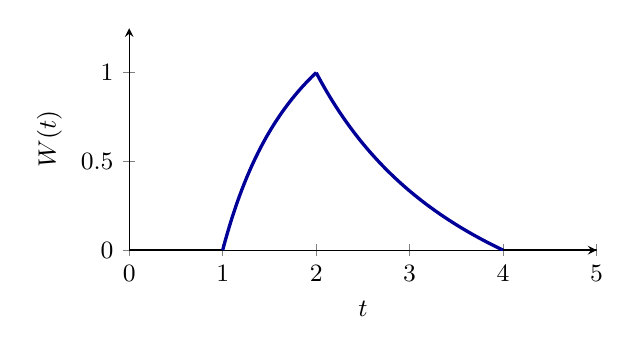
\begin{tikzpicture}
\begin{axis}[width=0.62\textwidth, height=4.4cm, xmin=0, xmax=5, ymin=0, ymax=1.25,
  xlabel={$t$}, ylabel={$W(t)$}, axis lines=left, tick label style={font=\small},
  label style={font=\small}, xtick={0,1,2,3,4,5}, ytick={0,0.5,1}]
  \addplot[black, thick, domain=0:1, samples=2] {0};
  \addplot[blue!60!black, very thick, domain=1:2, samples=40] {2*(1-1/x)};
  \addplot[blue!60!black, very thick, domain=2:4, samples=60] {4/x-1};
  \addplot[black, thick, domain=4:5, samples=2] {0};
\end{axis}
\end{tikzpicture}
\caption{The tent weight $W$ of Lemma~\ref{lem:tent}. Its integral is $2\log 2$.}
\label{fig:tent}
\end{figure}

\section{The transfer of pole data}\label{sec:transfer}

The upstream criterion works with the following package of hypotheses. It is the structure
\lean{PoleData} of~\cite{upstream}, copied in \lean{DelayedPoleSurvival.lean}.

\begin{definition}[Pole data]\label{def:poledata}
Let $g\colon\R\to\R$, $\Phi\colon\C\to\C$ and $Z\subset\C$. The triple $(g,\Phi,Z)$ is
\emph{pole data} if:
\begin{enumerate}
\item $g$ is measurable, and $|g(u)|\le Ce^{2u}$ for all $u\ge0$, for some $C$;
\item $\Phi(s)=\int_0^\infty g(u)e^{-su}\dd u$ for $\re s>2$;
\item every $\rho\in Z$ has $\re\rho>0$;
\item $\Phi$ is complex differentiable on $\{\re s>0\}\setminus Z$ (in the sense of
differentiability within that set);
\item for every $z$ with $\re z>0$ there is a punctured neighbourhood of $z$ disjoint from $Z$;
\item for every $\rho\in Z$ there are $r\ne0$ and $h$ analytic at $\rho$ with
$\Phi(s)=\tfrac r{s-\rho}+h(s)$ on a punctured neighbourhood of $\rho$; and if $\rho$ is real then
$r>0$.
\end{enumerate}
\end{definition}

\begin{theorem}[Crossley \cite{Crossley-transfer}; \lean{compactDifference\_poleData}]\label{thm:transfer}
Let $(g,\Phi,Z)$ be pole data and assume $\re\rho<1$ for every $\rho\in Z$. Then
$(\M g,\ m\Phi,\ Z)$ is pole data. For each $\rho\in Z$ the new residue is $m(\rho)$ times the old one.
\end{theorem}

\begin{proof}
(1) Each $\tau_ag$ is measurable, as the product of the indicator of $(a,\infty)$ with a
translate of $g$; the growth bound, with the constant $6C$, is in Proposition~\ref{prop:symbol}.
(2) is Proposition~\ref{prop:symbol}. (3) and (5) concern $Z$ only. (4) holds because $m$ is entire.
(6) For $\rho\in Z$ we have $0<\re\rho<1$, so Theorem~\ref{thm:pole} gives the expansion of
$m\Phi$ with residue $m(\rho)r\neq0$, and $m(\rho)r>0$ when $\rho$ is real.
\end{proof}

\begin{remark}[Why the poles are needed]\label{rem:landau}
A classical theorem of Landau states that the Laplace transform of a function of one sign is
analytic on the real axis to the right of a real singularity that it must possess at its abscissa
of convergence; see \cite[\S15.1]{MV}. Criteria of Landau type use this to pass from a one-sided
bound for $g$ to the absence of singularities of $\Phi$ with large real part. In the source
release~\cite{upstream}, the theorem \lean{landau\_window} has this form, as it is used
in~\cite{Crossley-transfer}: for pole data $(g,\Phi,Z)$, $0<\theta<1$ and $\delta>0$, a one-sided
window hypothesis on $g$ with exponent $\theta$ implies $\re\rho\le\theta$ for all $\rho\in Z$.
Theorem~\ref{thm:transfer} allows one to apply it to $\M g$ in place of $g$ with the same set $Z$.
If the mix had removed a pole, the conclusion for that point of $Z$ would have been lost. We do not
prove or use the Landau window theorem here.
\end{remark}

\section{A worked example}\label{sec:example}

Let $\rho_1=\tfrac12+i\gamma_1$, $\gamma_1=14.134725141734\ldots$, be the first zero of $\zeta$ in
the upper half-plane; it is a simple zero. All values below are rounded to six decimals.
\begin{center}
\begin{tabular}{@{}ll@{}}
\toprule
quantity & value\\
\midrule
$q=2^{-\rho_1}$ & $-0.658571+0.257458\,i$\\
$|q|=2^{-1/2}$,\quad $\arg q$ & $0.707107$,\quad $158.648^\circ$\\
$1-q$ & $\phantom{-}1.658571-0.257458\,i$\\
$2q-1$ & $-2.317141+0.514916\,i$\\
$m(\rho_1)=(1-q)(2q-1)$ & $-3.710574+1.450591\,i$\\
$|m(\rho_1)|$ & $3.984040$\\
bounds of Proposition~\ref{prop:bounds} at $\sigma=\tfrac12$ & $0.121320\le|m|\le4.121320$\\
$\res_{\rho_1}\Phi=1/(\tfrac14+\gamma_1^2)$ (Example~\ref{ex:zeta}) & $0.004999$\\
$|\res_{\rho_1}m\Phi|$ & $0.019916$\\
\bottomrule
\end{tabular}
\end{center}
The angle is $-\gamma_1\log2=-9.797445$ radians, which is $158.648^\circ$ modulo $360^\circ$. So
$q$ is close to the negative real axis, where $|m|$ is largest, and the residue at $\rho_1$ grows by
a factor close to $4$. For the next two zeros, $\gamma_2=21.022040$ and $\gamma_3=25.010858$, the
factors are $|m(\rho_2)|=2.962691$ and $|m(\rho_3)|=2.006492$ (Figure~\ref{fig:critical}).
The smallest possible factor on the critical line is $0.121320$, attained only at the points
$\tfrac12+2\pi ik/\log2$; whether a zero of $\zeta$ lies near such a point is a question about
$\gamma\log 2$ modulo $2\pi$, on which nothing is claimed here.

In the film these numbers appear as follows. The delayed tone is ``turned by $159$ degrees and
shrunk to $0.707$''; the three arrows $-1$, $3q$, $-2q^2$ placed head to tail leave a gap of length
$3.98$; the surface $|m|$ over the strip has a pillar of height $3.984$ at $\rho_1$; and the inset
graph is $\varphi$, with the value $0.121$ at $\sigma=\tfrac12$.

\section{Formal verification}\label{sec:lean}

The file \lean{DelayedPoleSurvival.lean} (namespace \lean{PrimeWindow}) imports only Mathlib. It was
checked with Lean~4.33.1 and Mathlib revision \lean{0df444a}, the versions pinned
by~\cite{Crossley-transfer}. Every theorem depends only on the axioms \lean{propext},
\lean{Classical.choice} and \lean{Quot.sound}.

\begin{center}
\footnotesize
\begin{tabular}{@{}p{0.23\textwidth}p{0.36\textwidth}p{0.34\textwidth}@{}}
\toprule
statement & Lean name (our file) & in \cite{Crossley-transfer}\\
\midrule
Lemma~\ref{lem:delay} & \lean{laplace\_delay} & \lean{laplace\_delay}\\
Proposition~\ref{prop:symbol} & \lean{laplace\_mix}, \lean{symbol\_expand} & inside the main proof\\
Proposition~\ref{prop:modes}, real $\lambda$ & \lean{mix\_exp}, \lean{mix\_const}, \lean{mix\_exp\_log\_two} & ---\\
Lemma~\ref{lem:radius} & \lean{norm\_q}, \lean{q\_mem\_annulus} & inside \lean{symbol\_strip}\\
Proposition~\ref{prop:zeros} & \lean{symbol\_ne\_zero}, \lean{symbol\_zero\_re}, \lean{symbol\_zero\_left}, \lean{symbol\_zero\_right} & \lean{symbol\_strip}\\
Proposition~\ref{prop:bounds}, lower bound & \lean{symbol\_norm\_lower}, \lean{floor\_pos} & ---\\
Corollary~\ref{cor:real} & \lean{symbol\_pos\_of\_real} & \lean{symbol\_real}\\
Lemma~\ref{lem:multiplier}, entire $M$ & \lean{pole\_transfer} & inside the main proof\\
Theorem~\ref{thm:pole} & \lean{pole\_survives\_mix}, \lean{residue\_norm\_lower} & ---\\
Lemma~\ref{lem:tent} & \lean{tent\_eq} & ---\\
Theorem~\ref{thm:transfer} & \lean{mix\_poleData} & \lean{compactDifference\_poleData}\\
\bottomrule
\end{tabular}
\end{center}

Not formalised in our file: the upper bound and the equality cases of
Proposition~\ref{prop:bounds}; the simplicity of the zeros and the ``only if'' direction of
Proposition~\ref{prop:zeros} in its exact form (the file proves that every zero has real part $0$
or $1$, and that the two progressions consist of zeros); Proposition~\ref{prop:mellin};
Example~\ref{ex:zeta}. The file has a floating-point layer that evaluates $q$, $m(\rho_1)$,
$\varphi(\tfrac12)$ and the minimum of $|m|/\varphi$ on a grid of the strip, and compares them with
the values of Section~\ref{sec:example}; this layer is a test, not a proof.

\section{Scope}\label{sec:scope}

This paper proves that the mix \eqref{eq:mix} preserves simple poles in the open strip, with
explicit control of the residues. It does not prove the Landau window theorem of~\cite{upstream},
it does not verify that a particular arithmetic function satisfies Definition~\ref{def:poledata},
and it does not prove a zero-free region. The criteria of
\cite{Crossley-transfer,Crossley-prime} are conditional statements: they derive a conclusion about
zeros from a hypothesis on windows that is not known to hold. Neither those criteria nor this paper
prove the Riemann hypothesis.

\begin{thebibliography}{9}

\bibitem{Crossley-transfer}
L.~Crossley, \emph{A delayed-difference window criterion for Dirichlet families}, Lean~4 source and
written proof, directory \texttt{results/dirichlet-window-transfer} of the repository
\url{https://github.com/leecrossley/prime-window-rh-criterion}, 2026.
DOI \href{https://doi.org/10.5281/zenodo.24410862}{10.5281/zenodo.24410862}. Licence CC~BY~4.0.

\bibitem{Crossley-prime}
L.~Crossley, \emph{An ordinary-prime window criterion for the Riemann hypothesis}, Lean~4 source and
written proof, \url{https://github.com/leecrossley/prime-window-rh-criterion}, 2026.
DOI \href{https://doi.org/10.5281/zenodo.24410878}{10.5281/zenodo.24410878}.

\bibitem{upstream}
Lean source release pinned by \cite{Crossley-transfer} (file
\texttt{LandauZeroFreeCriterion.lean}, definitions \lean{PoleData} and \lean{WindowHypU});
readable mirror at \url{https://github.com/Deicyde/riemann-hypothesis}, commit \texttt{40e56ba}.

\bibitem{Davenport}
H.~Davenport, \emph{Multiplicative Number Theory}, 3rd ed., revised by H.~L.~Montgomery,
Graduate Texts in Mathematics~74, Springer, 2000.

\bibitem{MV}
H.~L.~Montgomery and R.~C.~Vaughan, \emph{Multiplicative Number Theory I. Classical Theory},
Cambridge Studies in Advanced Mathematics~97, Cambridge University Press, 2007.

\bibitem{mathlib}
The mathlib Community, \emph{The Lean mathematical library}, in: Proceedings of the 9th ACM SIGPLAN
International Conference on Certified Programs and Proofs (CPP 2020), ACM, 2020, pp.~367--381.

\end{thebibliography}

\end{document}
